\documentclass[utf8]{ludis2022}


%%% Info Dokumenta pirmajai & dokumentārajai lapai
\fakultate{Eksakto zinātņu un tehnoloģiju}
\katedra{Matemātikas nodaļa}
\nosaukums{Polimondu virknes un formālās valodas}
\darbaveids{Bakalaura} %dokumentarajai lapai
\DARBAVEIDS{BAKALAURA DARBS} 
\autors{Marta Rudzāte}
\studapl{mr18118}
\vaditajs{Dr. math. Andrejs Cibulis}
\recenzents{Emīls Kalugins}
\vieta{Rīga}
\gads{2026}

%%% Valodu atbalsts ir stila failā, kur galvenā valoda - latviešu, bet te var pievienot papildu valodas
\setotherlanguages{english, german}

%%% Darbam noderīgas pakas
\usepackage[table,xcdraw]{xcolor} %Ja lieto krāsu tekstu
%\usepackage{mathtools}
\sloppy %Neļauj formulām iziet ārpus paragrāfa
\usepackage{float}

% % Bibliogrāfijai:
% \usepackage[style=plain, maxbibnames=99]{biblatex} %Imports biblatex package
% % Savieno autorus litertūras sarakstā
% \DeclareDelimFormat{finalnamedelim}{\addspace un\space}
% % \bibliographystyle{plain}
% \addbibresource{litsaraksts.bib} %Import the bibliography file
% \usepackage[style=plain, maxbibnames=99]{biblatex}
% \DeclareDelimFormat{finalnamedelim}{\addspace un\space}
% \addbibresource{litsaraksts.bib}

% \usepackage[
% backend=biber,
% style=numeric,
% maxbibnames=99
% ]{biblatex}
% \addbibresource{litsaraksts.bib}
% %%% Te var pievienot matemātisko operatoru saīsnes
% \DeclareMathOperator*{\argmax}{arg\,max}

\usepackage{comment}
\usepackage{tabularx}
\usepackage{makecell}
\usepackage{tcolorbox}

% Packages by Kalvis
% \usepackage{xcolor}
\usepackage[normalem]{ulem}
\usepackage{amsmath,amssymb}
\usepackage{mathrsfs}
\newcommand{\Gram}[1]{\mathscr{G}_{#1}}

% \theoremstyle{plain}
% \newtheorem{theorem}{Teorēma}[section]
% \newtheorem{corollary}[theorem]{Secinājums}
% \theoremstyle{definition}
% \newtheorem{definition}[theorem]{Definīcija}

% ----- Custom proof ending symbol -----
\renewcommand{\qedsymbol}{$\blacksquare$}

% ----- Custom environment for lemma with white square -----
\newenvironment{apgalvojumsproof}
  {\renewcommand{\qedsymbol}{$\square$}\proof}
  {\endproof}





\usepackage{hyperref} %pdf hiperlinki un pareizi punkti. NEDZĒST!!!!!

\begin{document}
\maketitle
\newpage



\section*{Anotācija}

\firstparskip Darbs veltīts perfektu polimondu eksistences jautājumiem.
Darbā ir piedāvātas jaunas perfekto polimondu ģenerēšanas metodes, kas saistītas ar 
bezkonteksta un paralēlo bezkonteksta gramatiku lietojumiem.  Ir izveidotas vairākas datorprogrammas šo metožu praktiskai realizācijai, pievēršot uzmanību tam, vai veidotās konstrukcijas (lauztās līnijas) atgriežas sākumpunktā un vai nenotiek malu krustošanās.


\vspace{0.5cm}
\textbf{Atslēgas vārdi:} izogoni, polimino, polimondi, bezkonteksta gramatika, paralēlā bezkonteksta gramatika, atbalsta vektoru mašīnas.


\newpage

\section*{Abstract}
\begin{english}

\firstparskip The work is devoted to the questions of the existence of perfect polyiamonds.
The work proposes new methods of generating perfect polyiamonds, related to the applications of
context-free and parallel context-free grammars. Several computer programs were created for the practical implementation of these methods, paying attention to whether the constructed constructions (broken lines) return to the starting point and whether there is no edge intersection.

\vspace{0.25cm}
\textbf{Keywords:} isogons, polyomino, polyiamonds, context-free grammar, parallel context-free grammar, support vector machines.

\end{english}

\newpage

%Satura rādītājs
\renewcommand{\contentsname}{Satura rādītājs}
\tableofcontents

\newpage
\specnodala{Definīcijas}


% {\bf{1. definīcija.}} Par polimino (angl. {\em polyomino}) sauc plaknes figūru, kas sastāv no vienības kvadrātiem, kuri pievienoti 
% viens otram pa vesela garuma malām.

{\bf{1. definīcija.}}
Par polimino (angl. {\em polyomino}, [1]) sauc plaknes figūru, kas sastāv no vienības kvadrātiem, kuri pievienoti 
viens otram pa vesela garuma malām.


% \noindent
% {\bf{1. definīcija.}} Par polimondu (angl. {\em polyiamond}) sauc plaknes figūru, kas sastāv no regulāriem vienības trijstūriem, 
% kuri pievienoti viens otram pa vesela garuma malām.
\vspace{10pt}

\noindent
{\bf{2. definīcija.}}
Par polimondu (angl. {\em polyiamond}, [2]) sauc plaknes figūru, kas sastāv no regulāriem vienības trijstūriem, 
kuri pievienoti viens otram pa vesela garuma malām.


% \vspace{10pt}

% \noindent
% {\bf{2. definīcija.}} Ja daudzstūra (polimino vai polimonda) visi malu garumi, sākot ar vienu virsotni, iet 
% pēc kārtas augošā secībā no $1$ līdz $n$, tad tādu daudzstūri sauc par perfektu.

\vspace{10pt}

\noindent
{\bf{3. definīcija.}}
    Ja $n$-stūra (polimino vai polimonda) visi malu garumi, sākot ar kādu virsotni, iet 
pēc kārtas augošā secībā no $1$ līdz $n$, tad tādu daudzstūri sauc par perfektu [2].



% \vspace{10pt}
% \noindent
% {\bf{3. definīcija.}} Par $90$ grādu secīgu
% izogonu (angl. {\em serial isogon of 90 degrees}) sauc daudzstūri, kurš satur tikai taisnus leņķus, un kura malu garumi, sākot no kādas virsotnes, ir naturāli skaitļi augošā secībā no $1$ līdz $n$. Šādu daudzstūri sauc arī par goligonu (angl. {\em golygon}).

% \vspace{10pt}
\vspace{10pt}

\noindent
{\bf{4. definīcija.}}
Par $90$ grādu secīgu
izogonu (angl. {\em serial isogon of 90 degrees}, [7]) sauc daudzstūri, kurš satur tikai taisnus leņķus, un kura malu garumi, sākot no kādas virsotnes, ir naturāli skaitļi augošā secībā no $1$ līdz $n$. Šādu daudzstūri sauc arī par goligonu (angl. {\em golygon}).


% \noindent
% {\bf{4. definīcija.}} Par $60$ grādu secīgu izogonu (angl. {\em serial isogon with 60-degree angles}) sauc perfektu polimondu, kura visi iekšējie leņķi ir vai nu $60°$ vai $300°$. Šādu daudzstūri arī sauc par perfektu šaurleņķu polimondu. 

% \vspace{10pt}

\vspace{10pt}

\noindent
{\bf{5. definīcija.}}
    Par $60$ grādu secīgu izogonu (angl. {\em serial isogon with 60-degree angles}, [7]) sauc perfektu polimondu, kura visi iekšējie leņķi ir vai nu $60°$ vai $300°$. Šādu daudzstūri arī sauc par perfektu šaurleņķu polimondu. 
\vspace{10pt}

\noindent
{\bf{6. definīcija.}}
     Par $120$ grādu secīgu izogonu (angl. {\em serial isogon with 120-degree angles}, [7]) sauc perfektu polimondu, kura visi iekšējie leņķi ir vai nu $120°$ vai $240°$. Šādu daudzstūri arī sauc par perfektu platleņķu polimondu. 



% \noindent
% {\bf{5. definīcija.}} Par $120$ grādu secīgu izogonu (angl. {\em serial isogon with 120-degree angles}) sauc perfektu polimondu, kura visi iekšējie leņķi ir vai nu $120°$ vai $240°$. Šādu daudzstūri arī sauc par perfektu platleņķu polimondu. 


% \vspace{10pt}
\vspace{10pt}

\noindent
{\bf{7. definīcija.}} 
Par {\em perfektu lauztu līniju} sauc lauztu līniju
no $n$ posmiem, kuras 
posmi iet pa bezgalīgā trijstūru režģa līnijām un 
posmu garumi ir secīgi $n, n-1, \ldots, 1$.

\vspace{10pt}

\noindent
{\bf{8. definīcija.}}
Ja $v$ un $w$ ir divas virknes alfabētā 
$\{$a,b,c,d,e,f$\}$ (to pieraksta arī 
$v,w \in \{$a,b,c,d,e,f$\}^{\ast}$), tad
\begin{itemize}
\item $|v|$ apzīmē $v$ {\em garumu} jeb burtu skaitu, 
kam vienmēr izpildās $|v| \in \mathbf{Z}_{0+}$.
\item $\varepsilon$ apzīmē {\em tukšo virkni} jeb 
vienīgo virkni, kuras garums ir $0$.
\item $vw$ apzīmē virkņu $v,w$ {\em konkatenāciju}, 
kur tās raksta vienu pēc otras. 
\item $v^k$ apzīmē virkni $v$, kas uzrakstīta $k$ reizes. 
\end{itemize}





\newpage
\specnodala{Ievads}

\firstparskip Pirmo reizi perfekti polimondi ir apskatīti  1988. gadā, kad Lī Salovs ({\em Lee Sallows}) definēja $90$ grādu secīgu izogonu. Kopā ar Martinu Gardneru ({\em Martin Gardner}) uzrādījis konstrukciju perfektiem $8k$-stūru polimino, kur $k \geq 1$, kurus var pārveidot par perfektiem polimondiem. 


2022. gada ATEE ikgadējās konferences ``
Būt vai nebūt lieliskam izglītotājam'' (angl. {\em To be or not to be a great educator}) rakstu krājumā 
[4] ir uzrādītas perfektu polimondu konstrukcijas katram pāra malu skaitam $n\geq 6$, kā arī ir labi pamatots, ka polimonda galapunkts savienosies ar tā sākumpunktu, tomēr nav pamatots, kāpēc malas savstarpēji nekrustojas. 

Autores kursa darbā ir uzrādītas vairākas konstrukcijas nepāra skaita malu polimondiem, kā arī ir dots piemērs, shēma kā pamatot, ka polimonda galapunkts atgriezīsies tā sākumpunktā. Tomēr nav pamatots, ka konstrukcijas vienmēr dos korektus polimondus. 


Darba mērķis ir pierādīt eksistenci perfektiem polimondiem. Mērķa sasniegšanai tika izvirzīti šādi darba uzdevumi:

\vspace{-15pt}
\begin{enumerate}
\item iepazīties ar literatūru, kas pieejama par perfektiem polimondiem;
\vspace{-10pt}
\item uzlabot kursa darbā atrasto konstrukciju shēmas;
\vspace{-10pt}
\item uzrakstīt datorprogrammu, lai atrastu jaunas konstrukcijas;
\vspace{-10pt}
\item pierādīt konstrukciju korektumu.
\vspace{-10pt}
\end{enumerate}


Darbs sastāv no $6$ nodaļām, definīciju saraksta, ievada, secinājumiem, izmantotās literatūras saraksta, anotācijas latviešu un angļu valodā. Darbā iekļauta viena tabula, $27$ attēli un $8$ literatūras avoti.


\newpage

\section{Jaunumi polimondu pasaulē}



\firstparskip \ref{tab:tab1}. tabulā var redzēt perfekto polimondu skaitu līdz pat $26$ malām. Šie polimondi tika atrasti un saskaitīti ar datorprogrammu, kas balstās uz koka apstaigāšanas jeb 
{\em backtracking} algoritmu.


\begin{comment}

Šos polimondus var apskatīt  \href{https://kapsitis.github.io/polimondi/polyiamond_lists/}{GitHub mājaslapā}.\\
{\color{teal} Linkus visur vajag aizstāt ar parastu literatūras atsauci.}

    
\end{comment}


\begin{comment}
 

\begin{table}[H]
\centering
\caption{Perfekto polimondu skaits atkarībā no malu skaita}\label{tab:tab1}
\setlength{\tabcolsep}{5.1pt}
\begin{tabular}{!{\vrule width 1.5pt}l!{\vrule width 1.5pt}l|l|l|l|l|l|l|l|l|l!{\vrule width 1.5pt}}
\Xhline{1.5pt}
$\textbf{n}$            & $5$ & $6$    & $7$    & $8$     & $9$     & $10$     & $11$     & $12$      \\ \hline
\textbf{Skaits} & $1$        & $1$    & $2$    & $9$     & $3$     & $4$      & $21$     & $87$     \\ \Xhline{1.5pt}
$\textbf{n}$       & $13$        & $14$         & $15$         & $16$   & $17$   & $18$    & $19$    & $20$      \\ \hline
\textbf{Skaits} & $288$   & $477$ & $1335$       & $4026$ & $8599$ & $22326$ & $67068$ & $193445$     \\ \Xhline{1.5pt}
$\textbf{n}$    & $21$     & $22$        & $23$       & $24$         & $25$         & $26$   &   &     \\ \hline
\textbf{Skaits}  & $526694$ & $1464978$  & $4284617$ & $12621026$  & $35662687$ & $102848450$ & &   \\ \Xhline{1.5pt}
\end{tabular}
\end{table}

   
\end{comment}


{\color{blue}
\begin{table}[H]
\centering
\caption{Perfekto polimondu skaits atkarībā no malu skaita}\label{tab:tab1}
\setlength{\tabcolsep}{5.1pt}

\begin{tabular}{!{\vrule width 1.5pt}l!{\vrule width 1.5pt}c|c|c|c|c|c|c|c|c|c|c|c|c|c!{\vrule width 1.5pt}}
\Xhline{1.5pt}
$\mathbf{n}$ & $5$ & $6$ & $7$ & $8$ & $9$ & $10$ & $11$ & $12$ & $13$ & $14$ & $15$ & $16$ & $17$ & $18$ \\ \hline
\textbf{Skaits} & $1$ & $1$ & $2$ & $7$ & $3$ & $4$ & $21$ & $87$ & $228$ & $477$ & $1335$ & $4026$ & $8599$ & $22326$ \\ 
\Xhline{1.5pt}
\end{tabular}

\vspace{2mm}

\begin{tabular}{!{\vrule width 1.5pt}l!{\vrule width 1.5pt}c|c|c|c|c|c|c|c!{\vrule width 1.5pt}}
\Xhline{1.5pt}
$\mathbf{n}$ & $19$ & $20$ & $21$ & $22$ & $23$ & $24$ & $25$ & $26$ \\ \hline
\textbf{Skaits} & $67068$ & $193445$ & $526694$ & $1464978$ & $4284617$ & $12621026$ & $35662687$ & $102848450$ \\ 
\Xhline{1.5pt}
\end{tabular}

\end{table}
}


\subsection{Baltic Way 2025 olimpiādes uzdevums}

\firstparskip 2025.gada starptautiskajā komandu matemātikas olimpiādē \textit{Baltic Way} viens no uzdevumiem bija par perfektiem polimondiem: 


\begin{tcolorbox}[
    colback=white,
    colframe=black,
    boxrule=0.8pt,
    title=9.\ uzdevums,
    coltitle=black,
    colbacktitle=white
]
Par {\it{Baltijas polimondu}} sauksim $n$-stūri, kura malu garumi ir $n, n-1, \dots, 2, 1$  tieši šādā secībā un visi iekšējo leņķu lielumi ir $120^\circ$ vai $240^\circ$. 

Pierādīt, ka jebkuram Baltijas polimondam
$n$ dalās ar $6$.

\end{tcolorbox}


Ievērojam, ka {\it{Baltijas polimondi}} ir tas pats, kas $120$ grādu secīgi izogoni, jeb perfekti platleņķu polimondi. Sk. [7], kur formulēts līdzīgs rezultāts, kas \textit{Baltic Way} žūrijai 
tolaik nebija zināms.



Olimpiādes uzdevuma pierādījums sastāv no $3$ daļām:

\vspace{-10pt}

\begin{enumerate}
    \item Polimonda malu skaits dalās ar $2$.

    \vspace{-10pt}
    
    \item Polimonda kodējums, kas sākas ar burtu a, sastāv no burtu pāriem ab, af, cb, cd, ed, ef noteiktā secībā. Burtu attiecīgos virzienus var redzēt \ref{fig:cord1}. attēlā.

    \vspace{-10pt}
    
    \item Polimonda malu skaits dalās ar $3$.
\end{enumerate}


LU \href{https://bw2025.lu.lv/izvelne-nr-2/problems-and-solutions/}{mājaslapā} var atrast pilnu pierādījumu.



\begin{figure}[H]
\center
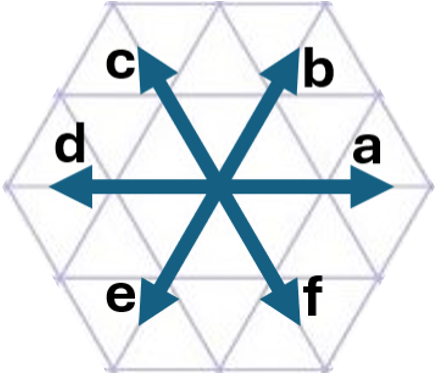
\includegraphics[width=5cm]{bildites/cordinates3.png}
\caption{Koordinātu sistēma trijstūru režģī}\label{fig:cord1}
\end{figure}





\section{Bezkonteksta gramatikas}

\firstparskip Rakstā [6] bezkonteksta gramatika (angl. {\em context-free grammar}, CFG) $G$ ir definēta kā četru elementu kopa: $G=(V, T, P, S)$, kur $V$ ir netermināļu (angl. {\em non-terminals}) kopa, $T$ ir termināļu (angl. {\em terminals}) kopa, $P$ ir produkciju (angl. {\em production rules}) kopa un $S \in V$ ir sākuma simbols. Valodas, kuras ir ģenerētas no bezkonteksta gramatikām, sauc par bezkonteksta valodām (angl. {\em context-free languages}, CFL).


Termināļi ir simboli, kas veido valodas elementus, un netermināļi palīdz izveidot šos elementus. Nosacījumi sastāv no trīs daļām: viena netermināļa, simbola ``$\rightarrow$'', termināļu un netermināļu virknītes, kas var būt arī tukša -- bez neviena simbola. Pielietojot šo produkciju, netermināli aizstāj ar virknīti, kas seko pēc bultas.  

\subsection{Polimondu iegūšana ar bezkonteksta gramatiku}




\firstparskip Pēc definīcijas, perfektai lauztai līnijai nav obligāti jābūt vienkāršai; tā 
ir nogriežņu secība 
$A_0A_1,\ A_1A_2,\ \ldots,\ A_{n-1}A_n$, 
kurā ir atļauta posmu savstarpēja krustošanās, 
tās pašas virsotnes izmantošana vairākās vietās, 
jauna posma vilkšana caur citus posmus savienojošo 
virsotni vai arī viena un tā paša nogriežņa vai 
posma vilkšana atkārtoti. Tā var būt 
un var arī nebūt slēgta -- nav 
zināms, vai $A_0 = A_n$.  

\begin{comment}

\begin{itemize}
\item Piemēram, $(ca)^3$ apzīmē to pašu ko $cacaca$.
\item Katrai virknei $v$ ir konkatenācijas 
$v\epsilon = v$ un $\epsilon{}v = v$. Daudzos citos 
gadījumos $vw \neq wv$.
\end{itemize}

Eksistē bijektīva atbilstība starp virknēm 
$w$ alfabētā $\{ a,b,c,d,e,f \}$ un perfektām lauztām 
līnijām, kur katram burtam atbilstošajā virzienā 
velk posmus garumā $|w|$, $|w|-1$, $\ldots$, $1$. 

\end{comment}

\firstparskip Lai aprakstītu perfektu polimondu, var izmantot koordinātu sistēmu, kas attēlota \ref{fig:cord1}. attēlā. Tā kā var pieņemt, ka polimonds sākas ar garāko malu un turpinās dilstošā secībā, tad jebkuru perfektu polimondu var aprakstīt ar virzienu burtiem a,b,c,d,e,f vienā vienīgā veidā. Šie seši burti veido termināļu kopu $T= \{$a,b,c,d,e,f$\}$ bezkonteksta gramatikai, kas veido perfektus polimondus. Lielie burti treknajā rakstā $\mathbf{P}, \mathbf{S}, \mathbf{T}$
būs netermināļi, kuriem var lietot gramatikas produkcijas, 
iegūstot no tiem jaunus termināļus un netermināļus.
Citi mazie burti, piemēram $u,v,w,x,y,z,t$ apzīmēs 
termināļu virknes jeb {\em stringus}, kas var būt gan 
perfekti polimondi, gan arī perfektas lauztas līnijas. Eksistē bijektīva atbilstība starp virknēm 
$w$ alfabētā $\{$a,b,c,d,e,f$\}$ un perfektām lauztām 
līnijām, kur katram burtam atbilstošajā virzienā 
velk posmus garumā $|w|$, $|w|-1$, $\ldots$, $1$. 
\begin{itemize}
\item Piemēram, (ca)$^3$ apzīmē to pašu ko cacaca.
\item Katrai virknei $v$ ir konkatenācijas 
$v\epsilon = v$ un $\epsilon{}v = v$. Daudzos citos 
gadījumos $vw \neq wv$.
\end{itemize}





\ref{fig:konstr_871a}. attelā uzzīmētos polimondus var aprakstīt ar šādu virkņu izteiksmi:

$$s_k = \mathtt{abfbfdf(bfdf)}^k\mathtt{dedcd(cdcb)}^k\mathtt{cdcbc},$$

vai arī ar šādu bezkonteksta gramatiku:

$$\mathcal{G}_1: \left\{
\begin{array}{rcl}
\mathbf{S} &\to& \mathtt{abfbfdf}\,\mathbf{P}\,\mathtt{cdcbc} \\
\mathbf{P} &\to& \mathtt{bfdf}\,\mathbf{P}\,\mathtt{cdcb} \\
\mathbf{P} &\to& \mathtt{dedcd}
\end{array}
\right.$$


{
\centering{
            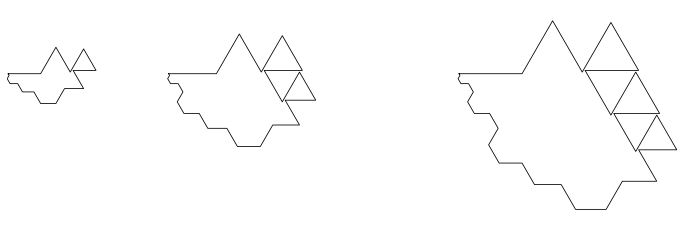
\includegraphics[width=\textwidth]{bildites/constr_8_7_1.png}
            \captionof{figure}{ ($8k+1$)-stūru perfektie polimondi, kur $k\geq 2$}
            \label{fig:konstr_871a}
}}











\begin{comment}


Rakstā \cite{cibulis_bulina} dotās perfekto polimondu konstrukcijas var aprakstīt ar bezkonteksta gramatikām. Piemēram, konstrukciju A, kura veido perfektu polimondu ar malu skaitu $n=8k+6$, kur $k\geq 0$, var aprakstīt šādi:

\vspace{0pt}


 
\noindent
\fbox{%
    \begin{minipage}{\textwidth}
            \bf{S} $\rightarrow$ \bf{P}$ fdb$\\
            \bf{P} $\rightarrow$ $cbcb $ \bf{P}$ fefe$ \\
            \bf{P} $\rightarrow$ $cae$
    \end{minipage}
}
   


$$\mathcal{G}_1: \left\{
\begin{array}{rcl}
\mathbf{S} &\to& \mathbf{P}\,\mathtt{fdb} \\
\mathbf{P} &\to& \mathtt{cbcb}\,\mathbf{P}\,\mathtt{fefe} \\
\mathbf{P} &\to& \mathtt{cae}
\end{array}
\right.$$

{\color{teal}
Manuprāt, gramatika $\mathcal{G}_1$ ir nepareiza. 
Sanāk, ka 
pats pirmais polimonds ir OK, bet 
turpmākie divi vairs neatgriežas 
uz sākumu: 
\begin{verbatim}
['caefdb', 'cbcbcaefefefdb', 'cbcbcbcbcaefefefefefdb']
[6, 14, 22]
WARNING: Polyiamond CBCBCAEFEFEFDB is not valid: 
    line segments do not close!
WARNING: Polyiamond CBCBCBCBCAEFEFEFEFEFDB is not valid: 
    line segments do not close!
\end{verbatim}

Varbūt domātas šādas bildītes? Tās ir no Jūsu 
kursa darba, bet 
pagrieztas un apsviestas, lai sāktos ar "AB" vai "AC", 
nevis ar malu virzienā "C".

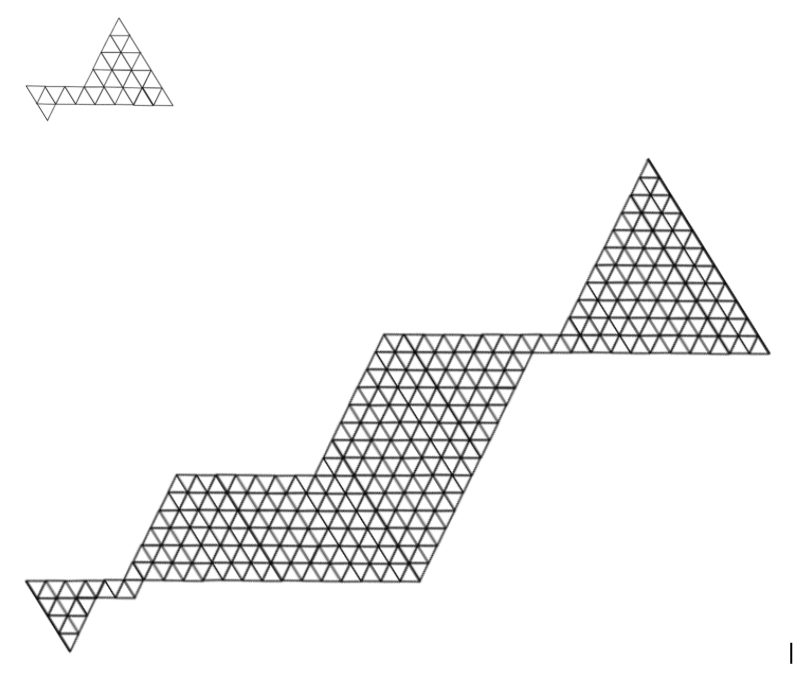
\includegraphics[width=4in]{draft_by_kalvis.png}

Priekš piemēriem zīmējumā (sk. augstāk) 
vajadzīga paralēlā gramatika, jo jaunas malas 
iesprauž trīs vietās:

$$\mathcal{G}_3: \left\{
\begin{array}{ccl}
\mathbf{S} &\to& \mathbf{P}_1\,\mathtt{ace}\,\mathbf{P}_2\,\mathtt{dfb}\,\mathbf{P}_1 \\
(\mathbf{P}_1,\; \mathbf{P}_2) &\to& (\mathbf{P}_1\,\mathtt{ab},\; \mathbf{P}_2\,\mathtt{dede}) \\
(\mathbf{P}_1,\; \mathbf{P}_2) &\to& (\varepsilon,\; \varepsilon)\\
\end{array}
\right.$$

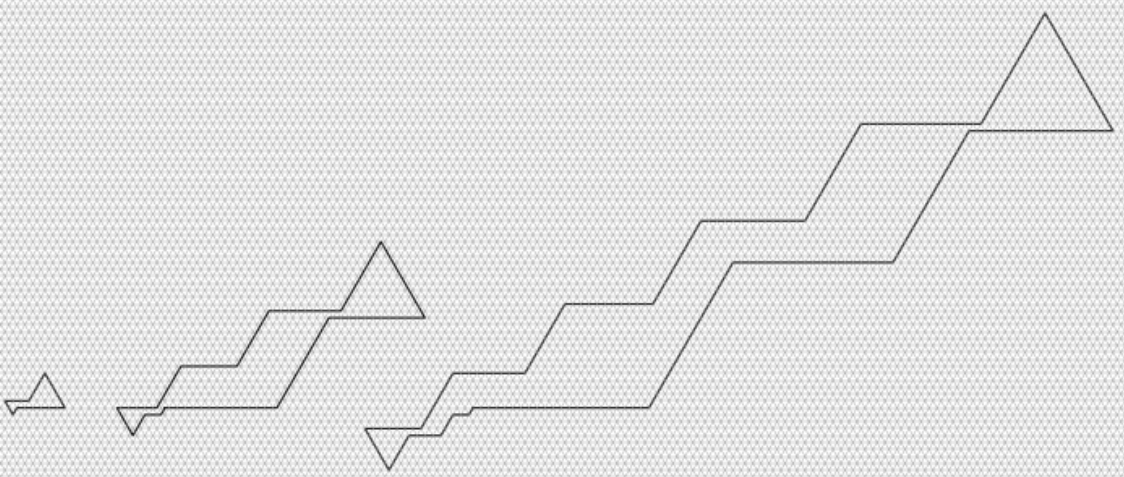
\includegraphics[width=6in]{8k_plus_6.png}

Manuprāt, šo piemēru var paturēt, bet nolikt 
kaut kur pie paralēlajām bezkonteksta gramatikām, 
bet parastajām bezkonteksta gramatikām šajā 
nodaļā paņemt 
citu piemēru - Jums jau Antigravity tādus uztaisīja.
}

    
\end{comment}


Ja ir vairākas produkcijas $\mathbf{P} \to \ldots$, tad gramatikas lietotājs var 
izvēlēties kuru produkciju lietot. 
Daudzi autori raksta 2.\ un 3.\ 
produkcijas vienā rindā, atdalot ar 
vertikālu svītriņu: 

$$\mathbf{P} \;\to\; \mathtt{bfdf}\,\mathbf{P}\,\mathtt{cdcb} \;\mid\; \mathtt{dedcd}$$


Tiklīdz kā $\mathbf{P}$ pārvērš par 
$\mathtt{dedcd}$, ir iegūta pabeigta
virzienu burtu virkne bez netermināļiem, 
kura apraksta kārtējo polimondu. 

\vspace{10pt}


\section{Paralēlās bezkonteksta gramatikas}


\firstparskip Rakstā [8] ir definēta paralēlā bezkonteksta gramatika (angl. {\em parallel context-free grammar}, PCG), izmantojot bezkonteksta gramatiku $G = (V, T, P, S)$. $G$ ir paralēlā bezkonteksta gramatika, ja $\forall  w_1 \overset{G}{\implies} w_2$ un $\forall A \in V$, 
kur $w_1 = x_1Ax_2A ... Ax_r$, $w_2 = x_1\alpha x_2\alpha ... \alpha x_r$, $r \geq 1$, $A \to \alpha \in P$ 
un $x_1, \ldots, x_r$ nesatur $A$. Šī definīcija pasaka, ka visi virknes saturošie netermināļi ir vienlaikus jāaizstāj ar vieniem un tiem pašiem nosacījumiem. Valodu $L=L(G)$ sauc par paralēlo bezkonteksta valodu (angl. {\em parallel context-free language}, PCL), ja $L$ ir ģenerēta ar paralēlo bezkonteksta gramatiku $G$.

Paralēlā bezkonteksta gramatikā var saskatīt līdzības ar Lindenmaiera sistēmām (angl. {\em  Lindenmayer systems}) jeb L--sistēmām. Vienīgi L--sistēmās malu skaits parasti aug eksponenciāli, pazīstams piemērs ir Koha sniegpārsla. Koha sniegpārslas iterācijas, kas visi arī ir (neperfekti) 
polimondi ģenerē šāda paralēlā gramatika (katrā nākamajā 
iterācijā netermināļu kļūst $4$ reizes vairāk): 

$$\mathcal{G}_{\text{Koch}}: 
\left\{ 
\begin{array}{ccl}
\bf{S} &\to& \mathtt{a}\bf{Z}\mathtt{c}\bf{U}\mathtt{e}\bf{W}\\

(\bf{Z}, \bf{T}, \bf{U}, \bf{V}, \bf{W}, \bf{X}) &\to& (\bf{Z}\mathtt{f}\bf{X}\mathtt{b}\bf{T}\mathtt{a}\bf{Z}, 
\bf{T}\mathtt{a}\bf{Z}\mathtt{c}\bf{U}\mathtt{b}\bf{T}, 
\bf{U}\mathtt{b}\bf{T}\mathtt{d}\bf{V}\mathtt{c}\bf{U},\\ 
 & & \bf{V}\mathtt{c}\bf{U}\mathtt{e}\bf{W}\mathtt{d}\bf{V},
\bf{W}\mathtt{d}\bf{V}\mathtt{f}\bf{X}\mathtt{e}\bf{W}, 
\bf{X}\mathtt{e}\bf{W}\mathtt{a}\bf{Z}\mathtt{f}\bf{X})\\
(\bf{Z}, \bf{T}, \bf{U}, \bf{V}, \bf{W}, \bf{X}) &\to& (\varepsilon, \varepsilon, \varepsilon, \varepsilon, \varepsilon, \varepsilon)\\
\end{array}
\right.
$$

{
\centering{
            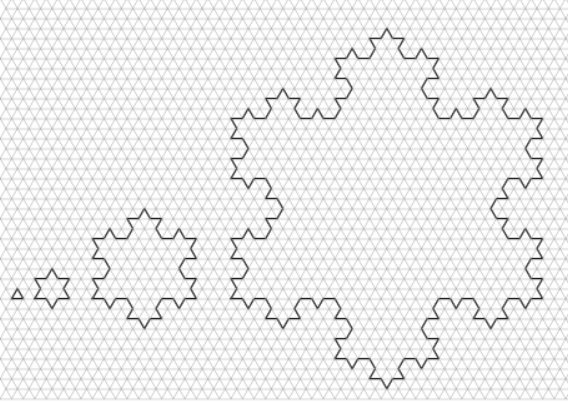
\includegraphics[width=4in]{koch_snowflake.png}
            \captionof{figure}{Koha sniegpārsla}
            \label{fig:coch}
}}



Atšķirībā no L-sistēmām, šajā darbā ieviestās paralēlās 
gramatikas nepalielina netermināļu skaitu un 
tāpēc polimonda malu skaits augs aritmētiskā 
progresijā.



\subsection{Polimondu iegūšana ar paralēlo bezkonteksta gramatiku}

\firstparskip Aplūkosim \ref{fig:konstr_85a}.attēlā attēloto konstrukciju. To var aprakstīt ar šādu paralēlo bezkonteksta gramatiku: 

\begin{comment}
    

\vspace{10pt}


\noindent
\fbox{%
    \begin{minipage}{\textwidth}
        \parbox{0.36\textwidth}{%  
            {\bf{S}} \to ~$a {\bf{P}}_1\ cacd\ {\bf{P}}_2\ e\ {\bf{P}}_2\ fdfdfa\ {\bf{P}}_1\ b$\\
            ${\bf{P}}_1 \to ca \ {\bf{P}}_1$\\
            ${\bf{P}}_2 \to fd \ {\bf{P}}_2$\\
        }
        \hfill
        \parbox{0.63\textwidth}{%
            \centering
            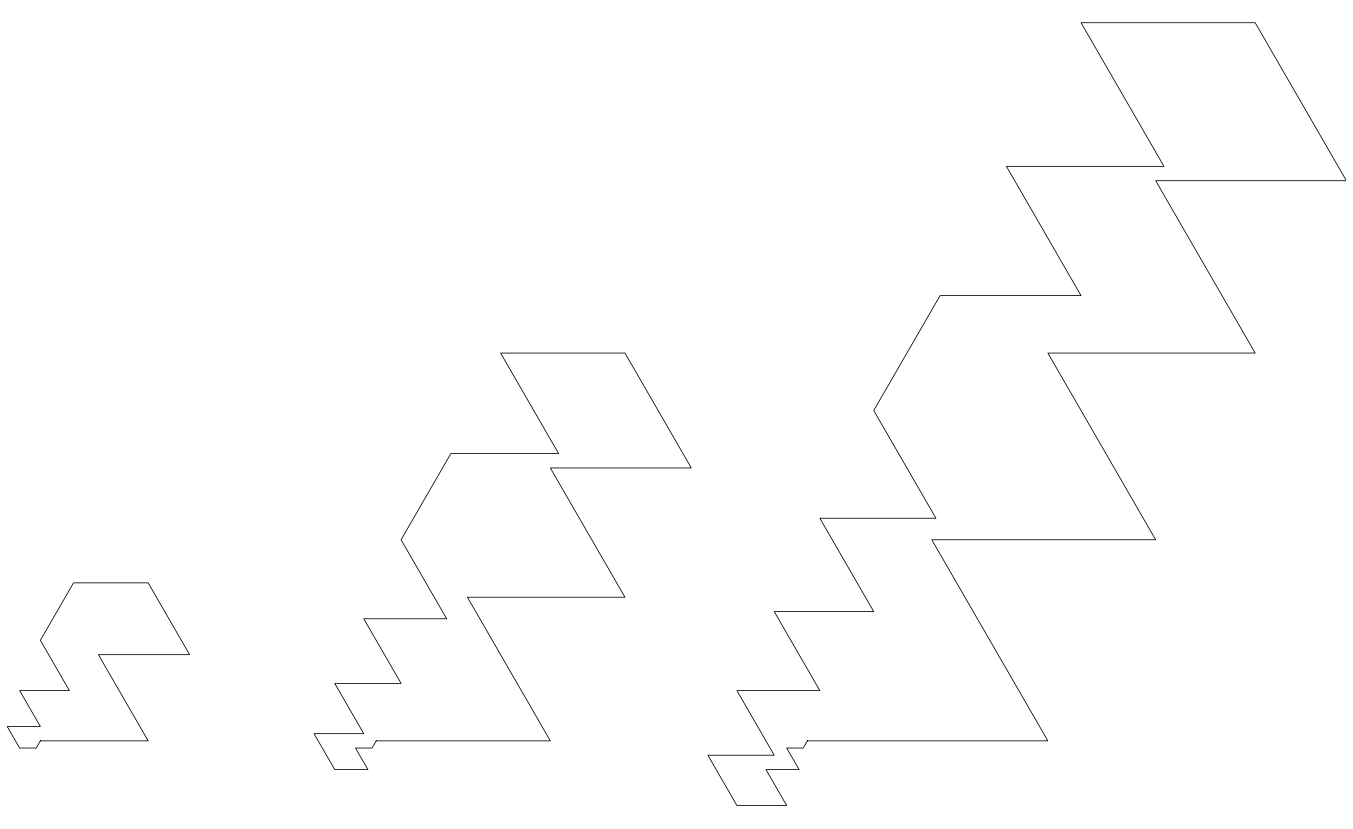
\includegraphics[width=0.63\textwidth]{bildites/konstr_85a.png}
            \captionof{figure}{ ($8k-3$)-stūru perfektie polimondi, kur $k\geq 2$}
            \label{fig:konstr_85a}
        }
    \end{minipage}
}

\vspace{10pt}

\end{comment}


$$\mathcal{G}_2: \left\{
\begin{array}{ccl}
\mathbf{S} &\to&
\mathtt{a}\,\mathbf{P}_1\,\mathtt{cacd}\,\mathbf{P}_2\,\mathtt{e}\,\mathbf{P}_2\,
\mathtt{fdfdfa}\,\mathbf{P}_1\,\mathtt{b}
\\
(\mathbf{P}_1,\; \mathbf{P}_2) &\to& (\mathtt{ca}\,\mathbf{P}_1,\; \mathtt{fd}\,\mathbf{P}_2)\\
(\mathbf{P}_1,\; \mathbf{P}_2) &\to& (\varepsilon,\; \varepsilon)\\
\end{array}
\right.$$



{
\centering{
            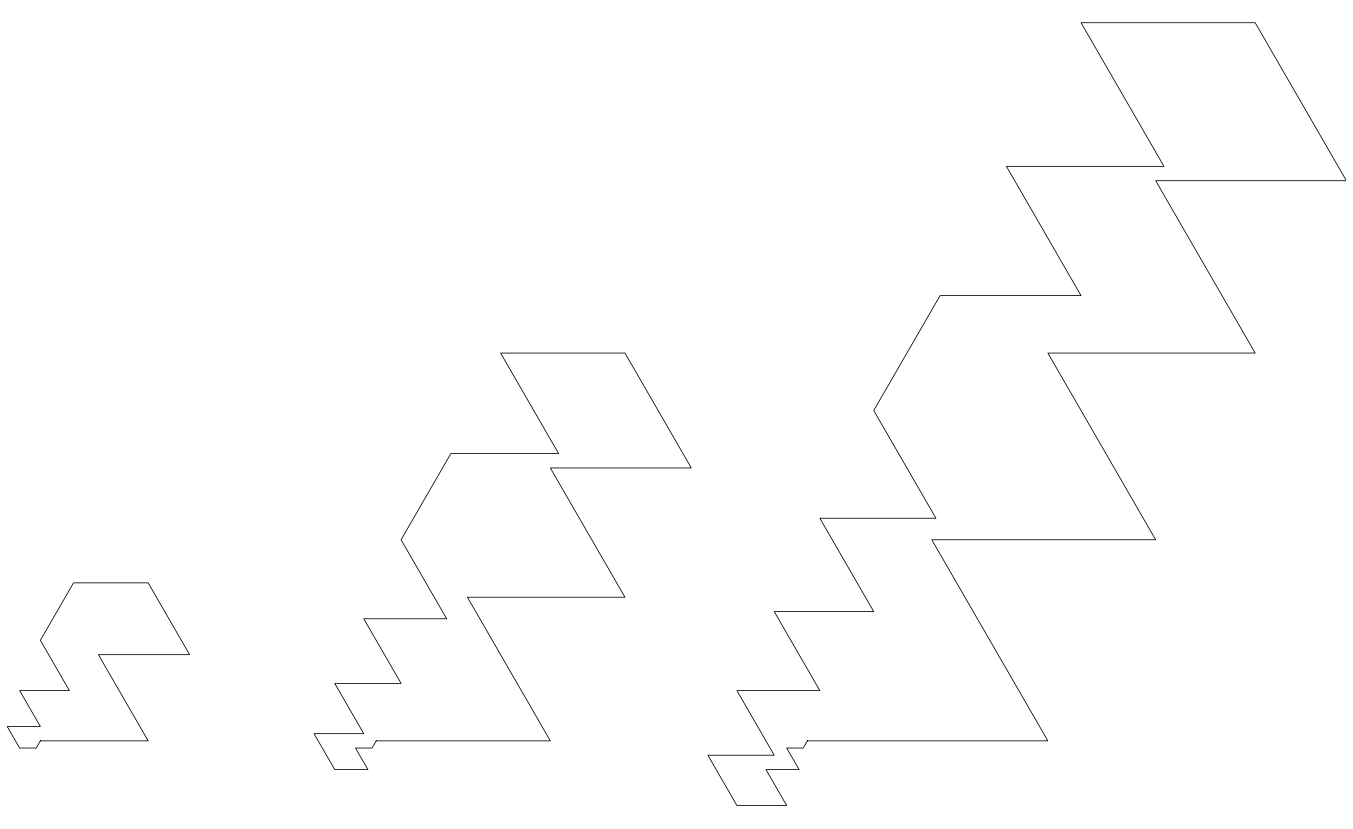
\includegraphics[width=\textwidth]{bildites/konstr_85a.png}
            \captionof{figure}{ ($8k-3$)-stūru perfektie polimondi, kur $k\geq 2$}
            \label{fig:konstr_85a}
}}


Šajā gadījumā produkciju kopa satur trīs 
likumus -- pirmais aiztāj sākumsimbolu 
$\mathbf{S}$ ar aksiomu, abi pārējie parāda, ko 
var darīt ``paralēli'' jeb vienlaikus ar netermināļiem $\mathbf{P}_1, \mathbf{P}_2$: 
\begin{itemize}
\item Vai nu $\mathbf{P}_1, \mathbf{P}_2$ vienlaikus pārveido attiecīgi par $\mathtt{ca}\,\mathbf{P}_1$ un 
$\mathtt{fd}\,\mathbf{P}_2$, 
\item Vai arī $\mathbf{P}_1, \mathbf{P}_2$ vienlaikus pārveido 
par tukšajām virknēm jeb izdzēš. 
Šajā gadījumā gramatikas produkcijas 
beidzas, jo visi netermināļi ir 
pazuduši. Un iegūtā virkne (cerams) 
iekodē kādu polimondu.
\end{itemize}


Daudzi autori otro un trešo likumu apvieno 
vienā rindā, atdalot abas izvēles ar vertikālu svītriņu:  
$$(\mathbf{P}_1, \mathbf{P}_2) \;\to\; (\mathtt{ca}\,\mathbf{P}_1,\ \mathtt{fd}\,\mathbf{P}_2) \;\mid\; (\varepsilon,\ \varepsilon)$$
Paralēlā gramatika šoreiz ir tikai 
formāls pieraksts, kā divās 
virknes vietās ``iepumpēt'' vienādā 
skaitā kaut kādas apakšvirknes.

Ērtības labad, konstrukciju varam arī pierakstīt šādi: 

\begin{equation}
s_k = \mathtt{a} (\mathtt{ca})^k \mathtt{cacd} (\mathtt{fd})^k \mathtt{e}(\mathtt{fd})^k \mathtt{fdfdfa} (\mathtt{ca})^k \mathtt{b}.
\label{eq:Sk}
\end{equation}




Ir spēkā pumpēšanas lemma bezkonteksta 
valodām ({\em Pumping lemma for context-free languages}), no kuras seko ka 
virknes $uv^nwx^ny$ (kur divas 
apakšvirknes $v$ un $x$ jāiesprauž 
vienādā skaitā) var iegūt 
ar bezkonteksta gramatikām, 
bet tādas virknes, kur vienādā skaitā 
iespraužamas trīs vai četras apakšvirknes -- vairs nav aprakstāmas ar bezkonteksta 
gramatikām. Tas paskaidro, kāpēc 
dažām polimondu konstrukcijām 
izmantotas parastas bezkonteksta gramatikas, bet citām -- parlēlās bezkonteksta 
gramatikas, jo tajās jaunas malu 
virknītes iespraužamas vairāk nekā divās vietās.


Ar bezkonteksta gramatikām un arī ar paralēlajām gramatikām var ģenerēt visdažādākās stringu kopas jeb {\em formālās valodas}.
Lai pārliecinātos, ka 
mūsu atrastās gramatikas ģenerē tikai perfektus polimondus
(nevis tikai perfektas lauztas līnijas), 
jāpārliecinās, ka perfektā lauztā līnija allaž 
atgriežas sākumpunktā (\ref{sect:construction_return}.\ nodaļa) un šīs lauztās līnijas posmi savstarpēji nepārklājas
(\ref{sect:no_intersects}.\ nodaļa).





\section{Konstrukcijas atgriešanās sākumpunktā}
\label{sect:construction_return}
\firstparskip 2024.gadā \href{https://conferences.lu.lv/event/493/contributions/2217/}{diskrētās matemātikas konferencē} prezentācijā ``Perfektu polimondu saimes un formālās valodas" (angl. {\it{``Families of Perfect Polyiamonds and Formal Languages"}}) tika prezentēts apgalvojums un teorēma, kas izcili pamato malu atgriešanos sākumpunktā konstrukcijām, kuras var aprakstīt ar bezkonteksta un paralēlajām bezkonteksta gramatikām. 

Visur zemāk izmantosim koordinātu sistēmu, kas ir attēlota \ref{fig:coord_2}. attēlā. 



{\centering{
            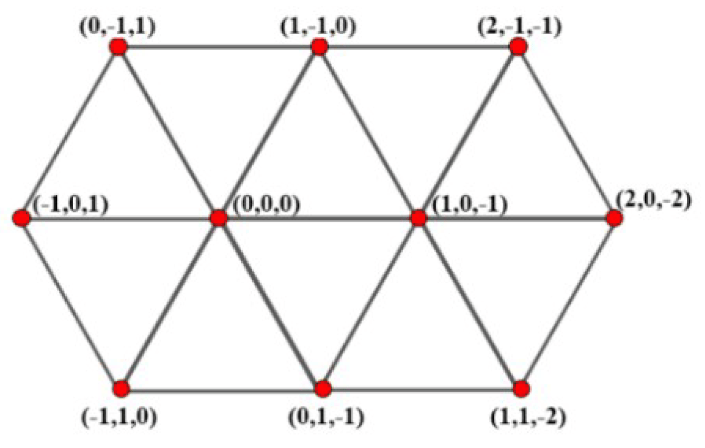
\includegraphics[width=0.55\textwidth]{bildites/cordinates1.png}
            \captionof{figure}{ Koordinātu sistēma}
            \label{fig:coord_2}
}} 


\begin{apgalvojums}\label{ap:1}
    
Doti $k$ vektori $u_1,  \dots, u_k$ un $k$ otrās pakāpes polinomi $P_i(t)$. Definējam
\[
v_n=\sum_{i=1}^k P_i(n)\cdot u_i.
\]
Tad visi $v_4, v_5, \dots $\  ir $v_1, v_2, v_3$ lineāras kombinācijas.
\end{apgalvojums}



\begin{apgalvojumsproof}
 Katram $n$ definējam koeficientus
\[
\alpha(n)=\frac{(n-2)(n-3)}{2}, \qquad
\beta(n)=-(n-1)(n-3), \qquad
\gamma(n)=\frac{(n-1)(n-2)}{2}.
\]

Tad $
v_n=\alpha(n)v_1+\beta(n)v_2+\gamma(n)v_3,
$ 
jo abas puses ir vienādi otrās pakāpes polinomi no $n$ ar vienādām vērtībām punktos $n=1,2,3$, un otrās pakāpes polinoms, kas sakrīt trijos punktos, ir viennozīmīgi noteikts.

\end{apgalvojumsproof}


\begin{teorema}\label{th:1}
Ja \   $s_n =
x_k y_k^{n} x_{k-1} y_{k-1}^{n} \cdots
x_2 y_2^{n} x_1 y_1^{n} x_0
$ \
ir perfekta slēgta lauzta līnija, kur
$
n = 1,2,3,
$
tad virzienu virkne $s_n$ apraksta perfektu polimondu
(vai vismaz perfektu lauztu līniju, kura ir slēgta -- atgriežas sākumpunktā)
visiem naturāliem $n$.
\end{teorema}
\begin{proof}

\begin{comment}
    


Ar $g(x_i)$ apzīmēsim visu virknītes $x_i$ virzienu vektoru summu, izmantojot garumus $|x_i|, |x_i-1|, \dots, 1$.
Ar $p(x_i)$ apzīmēsim visu $x_i$ virzienu vektoru summu, izmantojot garumus $1,1,...,1$. 

{\color{teal}
{\em Varbūt labāk ar summām nevis vārdiem. Piemēram:}
\end{comment}

Definējam jebkurai burtu 
virknītei $x=\mathtt{x}_1\ldots{}\mathtt{x}_L$ ar garumu $L = |x|$ 
šādas divas funkcijas, kuru vērtības ir vektori 
mūsu trijstūru režģa koordinātu sistēmā $\mathbb{Z}^3$:
\[
\begin{array}{rcl}
g(x) & = & \sum_{j = 1}^{L} (L - j + 1) \cdot \mathbf{h}(\mathtt{x}_j),\\
p(x) & = & \sum_{j = 1}^{L} \mathbf{h}(\mathtt{x}_j),\\
\end{array}
\]
kur $\mathbf{h}(\mathtt{x}_j)$ apzīmē
vienības vektoru $j$-tajam virziena burtam virknē $x$:
$\mathtt{x}_j \in \{ \mathtt{a}, \mathtt{b}, \mathtt{c}, \mathtt{d}, \mathtt{e}, \mathtt{f}\}$. Šie vienības vektori ir attiecīgi $\mathbf{h}(\mathtt{a}) = (1,0,-1)$, $\mathbf{h}(\mathtt{b}) = (1,-1,0)$, $\mathbf{h}(\mathtt{c}) = (0,-1,1)$, 
$\mathbf{h}(\mathtt{d}) = (-1,0,1)$, $\mathbf{h}(\mathtt{e}) = (-1,1,0)$, 
$\mathbf{h}(\mathtt{f}) = (0,1,-1)$.


Malu vektoru summa patvaļīgam $n$:
\[
v_n =
g(x_0)
+
\sum_{i=1}^{k}
\bigl(g(y_i)+g(x_i)\bigr)+
\]
\[
+
\sum_{i=1}^{k}
\left(
n\cdot |x_0|
+
\sum_{j=1}^{i-1}
n\cdot (n\cdot |y_j| + |x_j|)
+
\frac{n(n-1)}{2}|y_i|
\right)
\cdot v(y_i)+
\]
\[
+
\sum_{i=1}^{k}
\left(
|x_0|
+
\sum_{j=1}^{i-1}
(n\cdot |y_j| + |x_j|)
+
n\cdot |y_i|
\right)
\cdot v(x_i).
\]



\bigskip

Ar vektoriem $v_1,v_2,v_3$
var izteikt visus pārējos -- sk.\ref{ap:1}.\ apgalvojumu augstāk.
Ja $v_1,v_2,v_3=(0,0,0)$,
tad arī $v_4, v_5, ... =(0,0,0)$, t.i.\ visas lauztās līnijas
atgriezīsies sākumpunktā.

\end{proof}  











Piemērs ar paralēlo bezkonteksta gramatiku 
$\mathcal{G}_2$: 

\vspace{-10pt}

$$\left\{ 
\begin{array}{l}
g(\mathtt{acacdefdfdfab}) = 13\cdot(1,0,-1) + 12 \cdot (0,-1,1) + \ldots + (1,-1,0) = (0,0,0)\\
g(\mathtt{acacacdfdefdfdfdfacab}) = \ldots = (0,0,0)\\
g(\mathtt{acacacacdfdfdefdfdfdfdfacacab}) = \ldots = (0,0,0)\\
\end{array}
\right.$$

Tātad pirmās trīs lauztās līnijas 
gramatikas $\mathcal{G}_2$ ģenerētajā
virknē ir slēgtas. Pēc 
\ref{th:1}.~teorēmas arī visas 
turpmākās virknes
aprakstīs slēgtas
lauztas līnijas.

\subsection{120-grādu izogonu eksistence}

\firstparskip [7] apgalvots, ka ``secīgi 
120-grādu izogoni eksistē tad un tikai tad, ja 
$N$ dalās ar $6$''. 
Pierādijums, ka ikvienam secīgam 
$120^{\circ}$ izogonam malu skaits 
noteikti dalās ar $6$, dots 
{\em Baltic Way 2025} 9.uzdevuma 
atrisinājumā 
%\cite{BalticWay}. 
Šajā darbā pamatosim, ka visiem $n \geq 12$
dalāmība ar $6$ ir arī pietiekamais 
nosacījums. 
Tas pabeidz {\em Lee Sallows} apgalvojuma
pierādījumu, kurš pašā rakstā nav minēts.

\begin{apgalvojums}
Eksistē divas bezgalīgas 
perfektu platleņķu polimondu virknes, 
kuru malu garumi veido attiecīgi 
aritmētiskas progresijas $12, 24, 36,\ldots$
un $18, 30, 42, \ldots$ .
\end{apgalvojums}

\begin{apgalvojumsproof}
    

Aplūkosim polimondu virkni,
kas aprakstāma ar šādu
ar virkņu izteiksmi:
\[
(\mathtt{ab})^k\mathtt{abc}(\mathtt{de})^k\mathtt{de}(\mathtt{dc})^k\mathtt{de}(\mathtt{fa})^k\mathtt{fa}(\mathtt{fe})^k\mathtt{fa}(\mathtt{bc})^k\mathtt{b},\;\mbox{kur $k = 0,1,2,\ldots$}
\]
vai paralēlu bezkonteksta gramatiku
\[ 
\mathcal{G}_{12k+12}: \left\{ \begin{array}{ccl}
\mathbf{S} &\to& \mathbf{P}_1\,\mathtt{abc}\,\mathbf{P}_2\,\mathtt{de}\,\mathbf{P}_3\,\mathtt{de}\,\mathbf{P}_4\,\mathtt{fa}\,\mathbf{P}_5\,\mathtt{fa}\,\mathbf{P}_6\,\mathtt{b}\\
(\mathbf{P}_1,\,\mathbf{P}_2,\,\mathbf{P}_3,\,\mathbf{P}_4,\,\mathbf{P}_5,\,\mathbf{P}_6) &\to& (\mathbf{P}_1\mathtt{ab},\;\mathbf{P}_2\mathtt{de},\;\mathbf{P}_3\mathtt{dc},\;\mathbf{P}_4\mathtt{fa},\;\mathbf{P}_5\mathtt{fe},\;\mathbf{P}_6\mathtt{bc})\\
(\mathbf{P}_1,\,\mathbf{P}_2,\,\mathbf{P}_3,\,\mathbf{P}_4,\,\mathbf{P}_5,\,\mathbf{P}_6) &\to& (\varepsilon, \varepsilon, \varepsilon, \varepsilon, \varepsilon, \varepsilon)\\
\end{array} \right.
\]

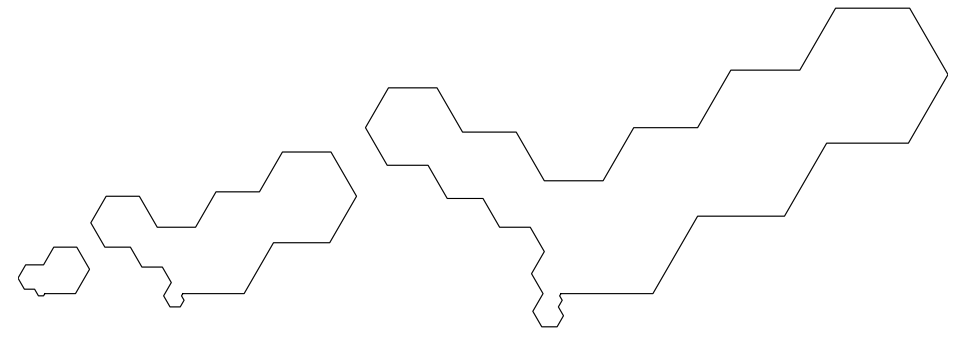
\includegraphics[width=6in]{120isogon_12_24_36.png}

Otru polimondu virkni
apraksta ar šādu
ar virkņu izteiksmi:

\[
(\mathtt{ab})^k\mathtt{abaf}(\mathtt{ed})^k\mathtt{eded}(\mathtt{ef})^k\mathtt{ed}(\mathtt{cb})^k\mathtt{cbcb}(\mathtt{cd})^k\mathtt{cb}(\mathtt{af})^k\mathtt{ab},\;\;\;\mbox{kur $k = 0,1,2,\ldots$}
\]


%un arī ar atbilstošu bezkonteksta 
%gramatiku $\mathcal{G}_{12k+18}$. 

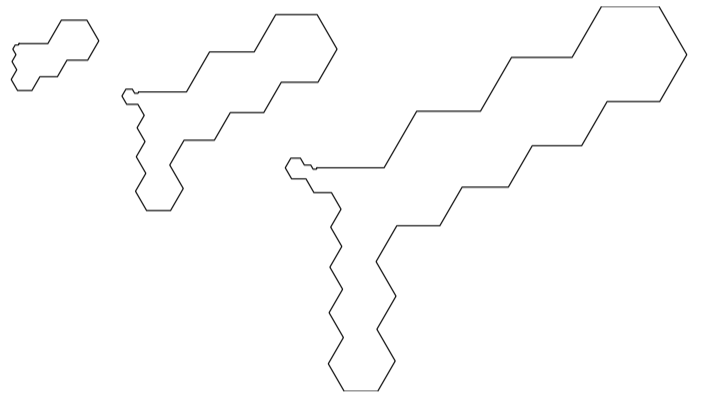
\includegraphics[width=6in]{120isogon_18_30_42.png}

Pārbaudot abās polimondu virknēs 
ietilpstošās burtu virknes, secinām, 
ka tajās vienmēr blakus atrodas 
burti $\mathtt{a} \leftrightarrow \mathtt{b}  \leftrightarrow \mathtt{c}  \leftrightarrow \mathtt{d}  \leftrightarrow \mathtt{e}  \leftrightarrow \mathtt{f}  \leftrightarrow \mathtt{a}$, kuru virzieni atšķiras 
tieši par $60^{\circ}$; tādēļ secīgās 
malas vienmēr veido $120^{\circ}$
leņķus. Turklāt, katrā no virknēm pirmie 
trīs locekļi apmierina \ref{th:1}.~teorēmas 
nosacījumu, t.i. arī visi turpmākie 
locekļi veido noslēgtas perfektas 
lauztas līnijas. 

\begin{comment}
  
Apsvērumi, kāpēc šajās perfektajās 
lauztajās līnijās posmi savstarpēji 
nekrustojas, izklāstīti \ref{sect:no_intersects}.~nodaļā. 
Ievērojam arī, ka malas sastāv no 
zigzagiem, kuri iet trīs dažādos 
virzienos un zigzagu joslas savstarpēji nepārklājas.
  
\end{comment}

\end{apgalvojumsproof}









\section{Malu nekrustošanās}
\label{sect:no_intersects}

\firstparskip Lai pierādītu perfektu polimondu eksistenci, ir arī jāpamato, ka atrastājām konstrukcijām malas nekrustojas. Lai gan daudzām konstrukcijām, skatoties uz polimondu bildītēm, nekrustošanās izskatās triviāli, tomēr apskatīsim metodi, iedvesmojoties no Neironu tīklos bieži apskatītā klasifikācijas uzdevuma - atbalsta vektoru mašīnas (angl. {\it{Support Vector Machines}}, SVM). 





\subsection{Atbalsta vektoru mašīnas pielietojums polimondiem}


\firstparskip Aplūkosim to pašu konstrukciju, kasir aprakstīta bezkonteksta gramatiku 
$\mathcal{G}_2$. 
Ar $\Gamma_k = \{\gamma_k = (\gamma_{k_1}, \gamma_{k_2}, \gamma_{k_3})\}$ aprakstīsim šīs gramatikas visu iegūto punktu kopu. No tās izvēlēsimies divus punktus: 

\vspace{-10pt}

$$P^+ = \gamma_k \;\mid\;  max\{\gamma_{k_1}+|\gamma_{k_2}|+|\gamma_{k_3}|\},$$ 

\vspace{-10pt}

$$P^- = \gamma_k \;\mid\;  min\{\gamma_{k_1}+|\gamma_{k_2}|+|\gamma_{k_3}|\}.$$

 $P^+$ ir augšējā labā virsotne, bet $P^-$ - apakšējā kreisā virsotne. Ar $\Gamma^-$ apzīmēsim $\Gamma_k$ apakškopu, kas sastāv no punktiem starp $P^+$ un $P^-$, bet ar $\Gamma^+$ apakškopu, kas sastāv no visiem pārējiem $\Gamma_k$ punktiem, izņemot $P^+$ un $P^-$. Ar $l^+$ un $l^-$ apzīmēsim lauzto līniju, ko veido attiecīgi $\Gamma^+$ un $\Gamma^-$. Parametrizēsim līnijas:
\[
l^+=(v_0,v_1,\dots,v_m),
\]
\[
l^-=(w_0,w_1,\dots,w_n),
\]
kur, ērtības labad, $v_i$ un $w_j$ ir koordinātas parastajā Dekarta sistēmā.

No gramatikas struktūras izriet sakarības:

\vspace{-10pt}

\begin{itemize}
    \item $ y(v_{i+1})\ge y(v_i),$
līdz ar to $l^+$ ir monotoni augoša ziemeļu virzienā, kas nozīmē, ka $l^+$ ir vienkārša. \
\item $ y(w_{i+1})\le y(w_i),$
kas nozīmē, ka $l^-$ ir monotoni augoša dienvidu virzienā, tādēļ arī $l^-$ ir vienkārša.

\end{itemize}



Tagad pielietosim atbalsta vektoru mašīnas ideju:

Definēsim funkciju
\[
h(v)=
\begin{cases}
+1,& v\in l^+,\\
-1,& v\in l^-,
\end{cases}
\]
un telpisko pacelšanu
\[
\Phi(v)=(x_v,y_v,h(v)).
\]

Tad:
\[
\Phi(l^+)\subset\{z=1\},
\qquad
\Phi(l^-)\subset\{z=-1\}.
\]

Ja plakne \(z=0\) pilnībā atdala abas lauztās līnijas trīs dimensijās, tad arī lauztā līnija no visiem $\Gamma_k$ punktiem ir vienkārša. Tā kā neviens nevēlas rēķināt visas $\Gamma_k$ punktu koordinātas ar roku, šai darbībai var izmantot datorprogrammu. 




\begin{comment}
    

Aplūkosim rekursīvi definētu slēgtu daudzstūra līkni
\[
\gamma_k ,
\]
kura tiek iegūta no gramatikas
\[
S(k)=a(ca)^kcad(fd)^ke(fd)^kfdfa(ca)^kb .
\]
Šī konstrukcija ģenerē tā sauktos \(8k\)-stūru perfektos polimondus.

Mērķis ir pierādīt, ka iegūtā robežlīkne ir vienkārša, t.i., tai nav paškrustojumu.

\subsection{Divu loku sadalījums}

Apzīmēsim ar
\[
P^- 
\]
apakšējo kreiso virsotni un ar
\[
P^+
\]
augšējo labo virsotni.

Izņemot šīs divas virsotnes, robežlīkne \(\gamma_k\) sadalās divos lokos:
\[
\gamma_k=\gamma^+\cup\gamma^- ,
\]
kur:

\begin{itemize}
    \item \(\gamma^+\) ir loks no \(P^-\) uz \(P^+\), ejot vienā virzienā;
    \item \(\gamma^-\) ir loks no \(P^-\) uz \(P^+\), ejot otrā virzienā.
\end{itemize}

Tādējādi
\[
\gamma^+\cap\gamma^- \supseteq \{P^-,P^+\}.
\]

Atliek parādīt, ka citu kopīgu punktu nav.

\subsection{Monotonitātes īpašība}

No gramatikas struktūras izriet, ka abi loki ir monotoni režģa ceļi.

Parametrizēsim lokus:
\[
\gamma^+=(v_0,v_1,\dots,v_m),
\]
\[
\gamma^-=(w_0,w_1,\dots,w_n),
\]
kur
\[
v_0=w_0=P^-,
\qquad
v_m=w_n=P^+.
\]

\subsubsection*{Augšējais loks}

Lokam \(\gamma^+\) katrā solī koordinātas apmierina:
\[
x(v_{i+1})\ge x(v_i),
\qquad
y(v_{i+1})\ge y(v_i),
\]
un vismaz viena nevienādība ir stingra.

Tātad loks \(\gamma^+\) ir monotoni augošs ziemeļaustrumu virzienā.

\subsubsection*{Apakšējais loks}

Savukārt lokam \(\gamma^-\):
\[
x(w_{j+1})\ge x(w_j),
\qquad
y(w_{j+1})\le y(w_j),
\]
un atkal vismaz viena nevienādība ir stingra.

Tātad loks \(\gamma^-\) ir monotoni augošs dienvidaustrumu virzienā.

\subsection{Kopīgo punktu neesamība}

Pieņemsim pretējo — eksistē iekšējs punkts
\[
q\in\gamma^+\cap\gamma^-,
\qquad
q\neq P^-,P^+.
\]

Tad eksistē indeksi \(i,j\), kuriem
\[
v_i=q=w_j,
\]
kur
\[
0<i<m,
\qquad
0<j<n.
\]

Tā kā loks \(\gamma^+\) ir ziemeļaustrumu monotons, visi tā turpmākie punkti apmierina:
\[
y\ge y(q).
\]

Savukārt lokam \(\gamma^-\), kas ir dienvidaustrumu monotons, visi turpmākie punkti apmierina:
\[
y\le y(q).
\]

Abi loki beidzas punktā \(P^+\), tādēļ jāizpildās:
\[
y(P^+)\ge y(q)
\]
un vienlaikus
\[
y(P^+)\le y(q).
\]

No tā seko:
\[
y(P^+)=y(q).
\]

Taču \(P^+\) ir vienīgā augstākā virsotne, tādēļ obligāti:
\[
q=P^+,
\]
kas ir pretruna ar pieņēmumu, ka \(q\) ir iekšējs punkts.

Tātad:
\[
\gamma^+\cap\gamma^-=\{P^-,P^+\}.
\]

\subsection{Pacelšana trīs dimensijās}

Definēsim funkciju
\[
h(v)=
\begin{cases}
+1,& v\in\gamma^+,\\
-1,& v\in\gamma^-,
\end{cases}
\]
un telpisko pacelšanu
\[
\Phi(v)=(x_v,y_v,h(v)).
\]

Tad:
\[
\Phi(\gamma^+)\subset\{z=1\},
\qquad
\Phi(\gamma^-)\subset\{z=-1\}.
\]

Plakne \(z=0\) pilnībā atdala abus lokus trīs dimensijās. Tā kā loki koplieto tikai galapunktus \(P^-\) un \(P^+\), tie nevar krustoties plaknē.

Līdz ar to robežlīkne \(\gamma_k\) ir vienkārša.



\end{comment}




    




\begin{comment}



\subsection{Vertikālās līnijas nekrustošana; taisnstūri}

{\color{blue}
{\em Lai varētu pierakstīt - var 
uzzīmēt no kādas virknes 
3 ērtus polimondus, un 
zigzagiem (kaut vai ar roku) 
apvilkt taisnstūrveida rāmīšus.

Var palūgt Antigravity izrēķināt 
taisnstūrveida rāmīšiem ierobežojošā
taisnstūra (bounding box) koordinātes; varbūt arī izteikt 
kā polinomu no $n$. 
Tad var pamatot nevienādību, 
ka viens taisnstūris neuzskrien 
virsū otram.
}
}

    
\end{comment}






\section{Pārējās konstrukcijas}

\firstparskip Iedodod aplikācijai ``Antigravity" visus iegūtos rezultātus, uzrakstītās programmatūras, visus perfektos polimondus līdz malu skaitam $26$,  izbūra jaunas konstrukcijas: ... 
šeit tekstu garāku no rīta uzrakstīšu :)

Zemāk esošajām bildēm nosaukumi zem attēla var būt nepareizi.

{
\centering{
            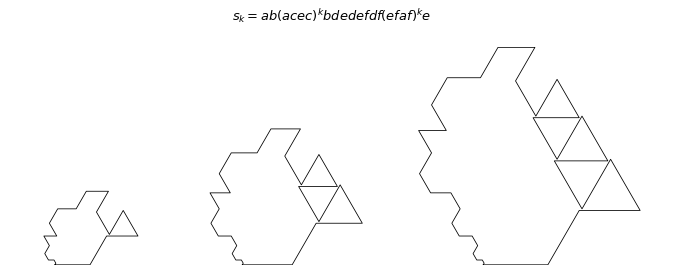
\includegraphics[width=\textwidth]{bildites/c1.png}
            \captionof{figure}{ ($8k+3$)-stūru perfektie polimondi, kur $k\geq 2$}
            \label{fig:c1}
}}

{
\centering{
            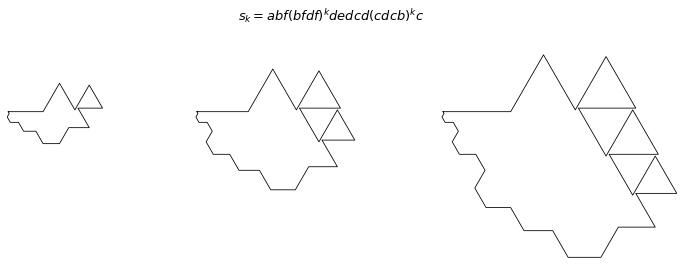
\includegraphics[width=\textwidth]{bildites/c2.png}
            \captionof{figure}{ ($8k+3$)-stūru perfektie polimondi, kur $k\geq 2$}
            \label{fig:c2}
}}

{
\centering{
            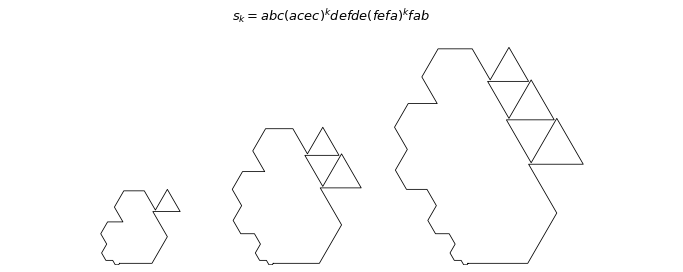
\includegraphics[width=\textwidth]{bildites/c3.png}
            \captionof{figure}{ ($8k+3$)-stūru perfektie polimondi, kur $k\geq 2$}
            \label{fig:c3}
}}


{
\centering{
            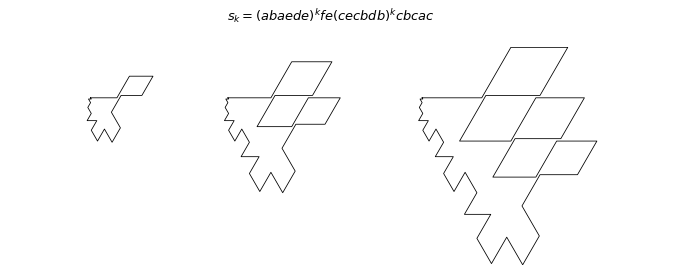
\includegraphics[width=\textwidth]{bildites/c4.png}
            \captionof{figure}{ ($8k+3$)-stūru perfektie polimondi, kur $k\geq 2$}
            \label{fig:c4}
}}

{
\centering{
            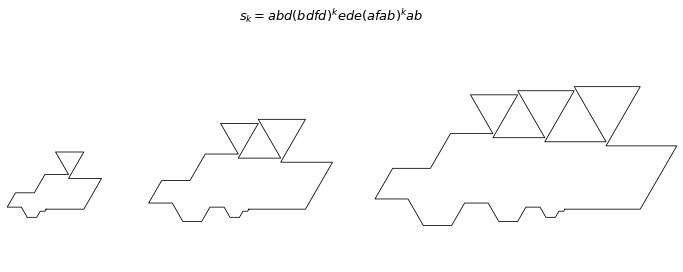
\includegraphics[width=\textwidth]{bildites/c5.png}
            \captionof{figure}{ ($8k+3$)-stūru perfektie polimondi, kur $k\geq 2$}
            \label{fig:c5}
}}


{
\centering{
            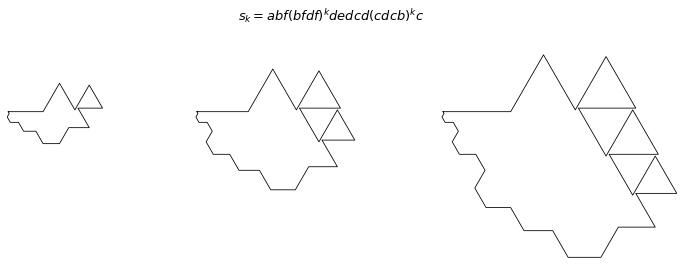
\includegraphics[width=\textwidth]{bildites/c6.png}
            \captionof{figure}{ ($8k+3$)-stūru perfektie polimondi, kur $k\geq 2$}
            \label{fig:c6}
}}

{
\centering{
            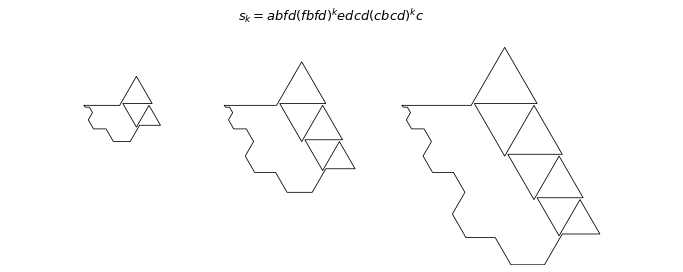
\includegraphics[width=\textwidth]{bildites/c7.png}
            \captionof{figure}{ ($8k+3$)-stūru perfektie polimondi, kur $k\geq 2$}
            \label{fig:c7}
}}

{
\centering{
            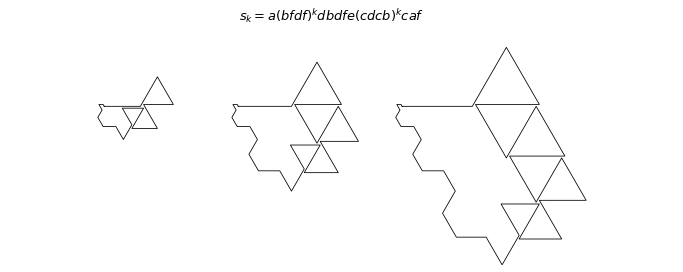
\includegraphics[width=\textwidth]{bildites/c8.png}
            \captionof{figure}{ ($8k+3$)-stūru perfektie polimondi, kur $k\geq 2$}
            \label{fig:c8}
}}

{
\centering{
            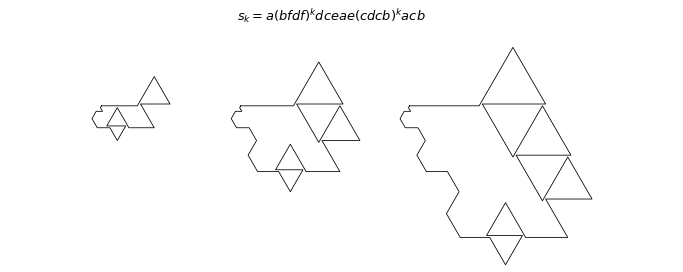
\includegraphics[width=\textwidth]{bildites/c9.png}
            \captionof{figure}{ ($8k+3$)-stūru perfektie polimondi, kur $k\geq 2$}
            \label{fig:c9}
}}

{
\centering{
            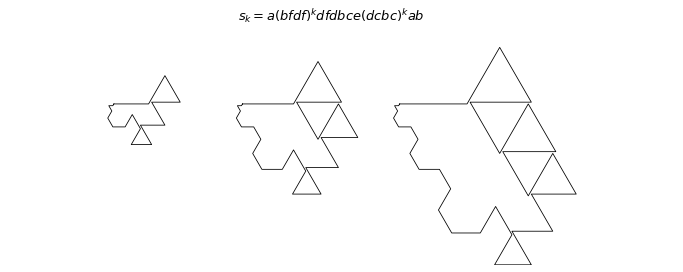
\includegraphics[width=\textwidth]{bildites/c10.png}
            \captionof{figure}{ ($8k+3$)-stūru perfektie polimondi, kur $k\geq 2$}
            \label{fig:c10}
}}

{
\centering{
            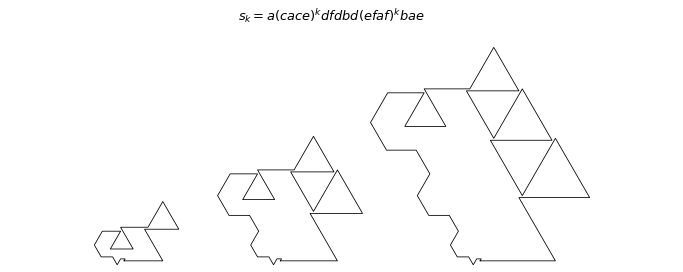
\includegraphics[width=\textwidth]{bildites/c11.png}
            \captionof{figure}{ ($8k+3$)-stūru perfektie polimondi, kur $k\geq 2$}
            \label{fig:c11}
}}

{
\centering{
            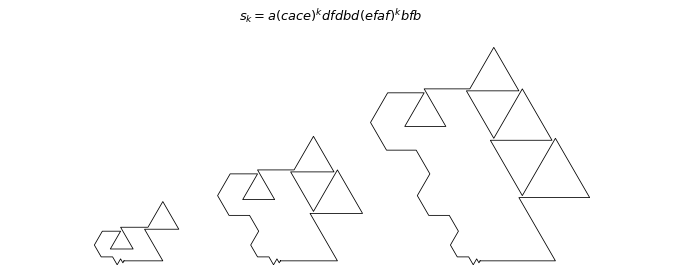
\includegraphics[width=\textwidth]{bildites/c12.png}
            \captionof{figure}{ ($8k+3$)-stūru perfektie polimondi, kur $k\geq 2$}
            \label{fig:c12}
}}

{
\centering{
            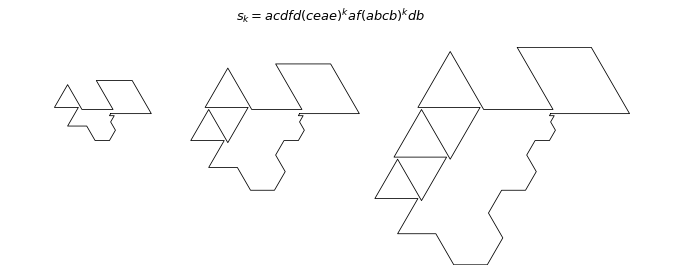
\includegraphics[width=\textwidth]{bildites/c13.png}
            \captionof{figure}{ ($8k+3$)-stūru perfektie polimondi, kur $k\geq 2$}
            \label{fig:c13}
}}

{
\centering{
            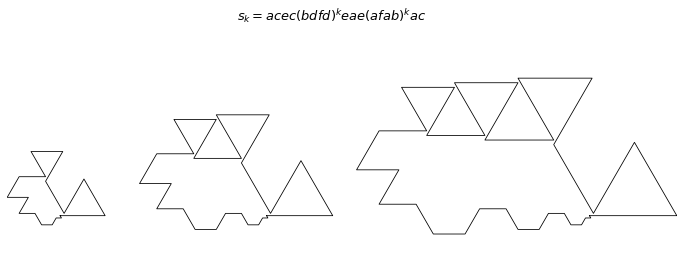
\includegraphics[width=\textwidth]{bildites/c14.png}
            \captionof{figure}{ ($8k+3$)-stūru perfektie polimondi, kur $k\geq 2$}
            \label{fig:c14}
}}

{
\centering{
            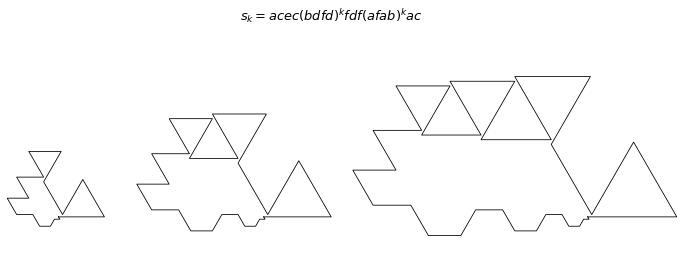
\includegraphics[width=\textwidth]{bildites/c15.png}
            \captionof{figure}{ ($8k+3$)-stūru perfektie polimondi, kur $k\geq 2$}
            \label{fig:c15}
}}
{
\centering{
            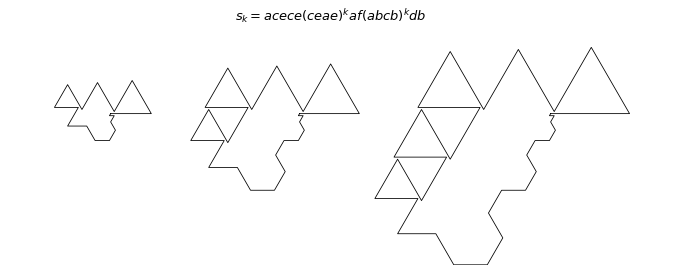
\includegraphics[width=\textwidth]{bildites/c16.png}
            \captionof{figure}{ ($8k+3$)-stūru perfektie polimondi, kur $k\geq 2$}
            \label{fig:c16}
}}
{
\centering{
            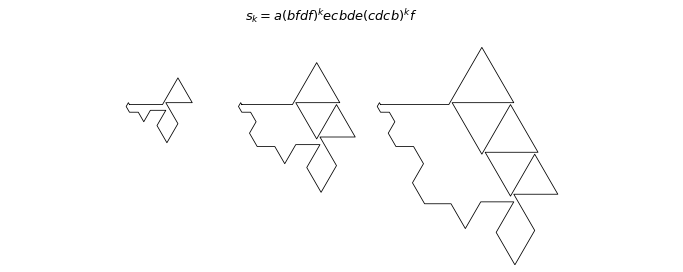
\includegraphics[width=\textwidth]{bildites/c17.png}
            \captionof{figure}{ ($8k+3$)-stūru perfektie polimondi, kur $k\geq 2$}
            \label{fig:c17}
}}

{
\centering{
            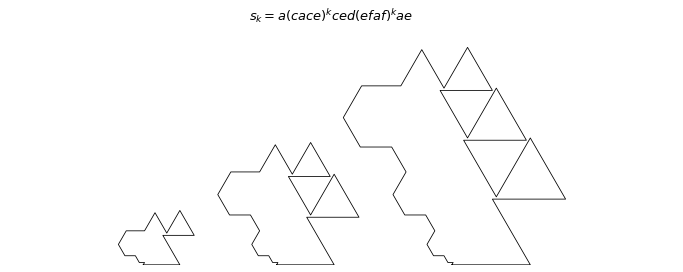
\includegraphics[width=\textwidth]{bildites/c18.png}
            \captionof{figure}{ ($8k+3$)-stūru perfektie polimondi, kur $k\geq 2$}
            \label{fig:c1}
}}

{
\centering{
            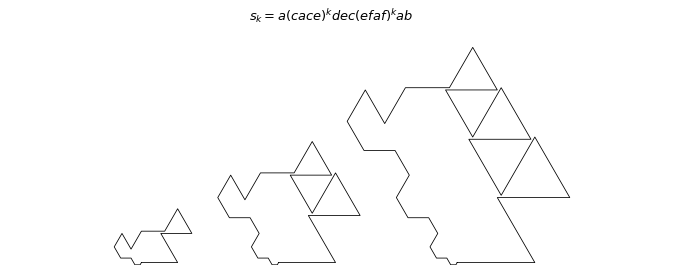
\includegraphics[width=\textwidth]{bildites/c19.png}
            \captionof{figure}{ ($8k+3$)-stūru perfektie polimondi, kur $k\geq 2$}
            \label{fig:c19}
}}

{
\centering{
            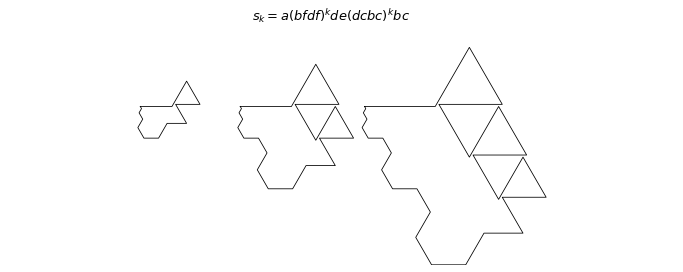
\includegraphics[width=\textwidth]{bildites/c20.png}
            \captionof{figure}{ ($8k+3$)-stūru perfektie polimondi, kur $k\geq 2$}
            \label{fig:c20}
}}

{
\centering{
            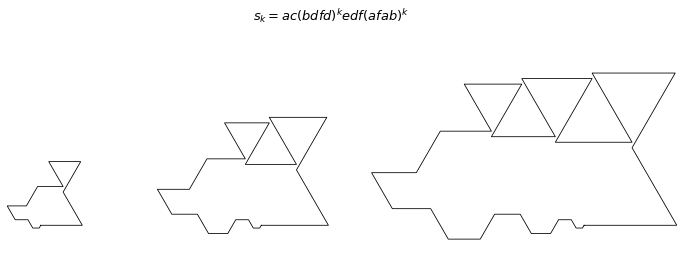
\includegraphics[width=\textwidth]{bildites/c21.png}
            \captionof{figure}{ ($8k+3$)-stūru perfektie polimondi, kur $k\geq 2$}
            \label{fig:c21}
}}

{
\centering{
            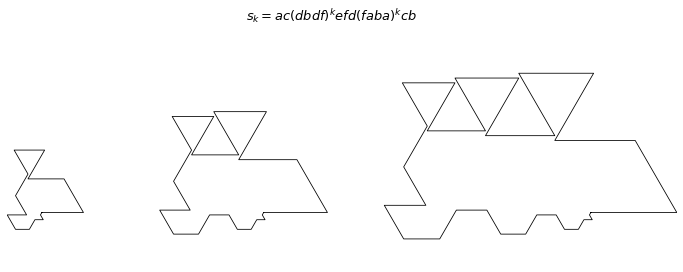
\includegraphics[width=\textwidth]{bildites/c22.png}
            \captionof{figure}{ ($8k+3$)-stūru perfektie polimondi, kur $k\geq 2$}
            \label{fig:c22}
}}




\newpage

\specnodala{Secinājumi}

\firstparskip
Uzsākot pētījumu par bezgalīgu polimondu 
virkņu eksistenci un to konstruēšanu tās sākotnēji prasīja iespraust jaunas malas -- parasti pa divām četrās dažādās vietās. 

Radās jautājumi par to, vai šādas 
konstrukcijas nav nevajadzīgi 
sarežģītas. Vai eksistē viegli 
definējamas un formāli pierakstāmas 
polimondu saimes, ar ko pamatot 
gan dažādu polimondu saimju eksistenci, 
gan arī iegūt novērtējumus to ģeometriskajām
īpašībām (piemēram, apakšējo novērtējumu 
maksimālajam laukumam, kas var būt 
perfektam $n$-stūru polimondam). 

Var formulēt dažādus grūti 
atbildamus jautājumus par perfektu 
polimondu saimēm. Piemēram,
Kuriem $n$ atradīsies tāds 
perfekts $n$-stūru polimonds, kurā var
iespraust vienu jaunu malu (atstājot 
iepriekšējo malu virzienus) tā, lai 
rastos perfekts $(n+1)$-stūru polimonds?
Vai eksistē tādas saimes, kur 
jaunas malas iesprauž nevis četrās 
vietās, bet tikai trīs, divās vai vienā?

2024.\ gada LU \href{https://conferences.lu.lv/event/493/contributions/2217/}{diskrētās matemātikas konferencē}(\url{https://docs.google.com/presentation/d/14KTTfThGzuGj3ykdrakvxId13KNMfYJWKHc5CAuD2eE/edit?usp=sharing}) 
tika pamatots, ka vienā vietā iespraužot, bezgalīga 
polimondu virkne nevar eksistēt, bet var panākt bezgalīgas
perfektu polimondu virknes, 
neierobežoti iespraužot jaunas malas 
divās (vai vairāk) vietās. 

Šajā bakalaura darbā šī ideja ir attīstīta 
tālāk, izveidojot gramatikas virknēm, kuru 
ģenerētie polimondi pēc malu skaita 
pārklāj visu pietiekami lielo 
$n \in \mathbb{N}$ kopu ($n \geq 17$). 
Malu skaitam $n \in [5;16]$ 
perfektos polimondus var atrast, neizmantojot 
virknes, bet lietojot pilno pārlasi 
(jeb precīzāk, ar koka apstaigāšanas jeb 
{\em backtracking} algoritmu).


Formālās valodas varētu izmantot ne vien eksistences 
pierādījumos, bet arī veidojot polimondu virknes 
ar noteiktām īpašībām. Piemēram, malu skaitam $n = 8k$
ar paralēlajām gramatikām var izveidot perfektus polimino 
(vai arī polimondus, ja koordinātu asis kopā ar attēlu 
sašķiebj $60^{\circ}$ leņķī), kam 
malas ietu pa trijstūru režģa līnijām) un tiem ir 
lielākais iespējamais diametrs starp visiem polimino 
(vai attiecīgi -- polimondiem). Līdzās diametram būtu 
svarīgi aplūkot arī laukumu un citus ģeometriskus raksturlielumus.






















\newpage


\clearpage

\section*{IZMANTOTĀ LITERATŪRA UN AVOTI}
\addcontentsline{toc}{section}{Izmantotā literatūra un avoti}

\begin{enumerate}
\renewcommand{\labelenumi}{[\arabic{enumi}]}

\item Elīna Buliņa.
\textit{Maģiskie daudzstūri un to īpašības}.
Bakalaura darbs, 2016.

\item Elīna Buliņa.
Maģiskie polimino un polimondi.
\textit{Vidzemes Augstskolas 11.\ studentu pētniecisko darbu konferences zinātnisko rakstu krājums},
7.--8.\ lpp., 2017.

\item Elīna Buliņa.
\textit{Maģiskie polimondi un to īpašības}.
Maģistra darbs, 2018.

\item Andrejs Cibulis un Elīna Buliņa.
Fostering Teachers’ Mathematical Competence in Problem Solving.
\textit{To be or not to be a great educator},
652--665, 2022.

\item Alexander Keewatin Dewdney.
An Odd Journey Along Even Roads Leads to Home in Golygon City.
\textit{Scientific American},
263(1):118--121, 1990.

\item John Hopcroft un Jefrey Ullman.
\textit{Introduction to Automata Theory, Languages, and Computations},
2006.

\item Lee Sallows, Martin Gardner, Richard Kenneth Guy un Donald Knuth.
Serial isogons of 90 degrees.
\textit{Mathematics Magazine},
64(5):315--324, 1991.

\item Rani Siromoney un Kamala Krithivasan.
Parallel context-free languages.
\textit{Information and Control},
24(2):155--162, 1974.

\end{enumerate}












\end{document}
